\documentclass[a4paper]{article}

\usepackage[utf8]{inputenc}
\usepackage[T1]{fontenc}
\usepackage{textcomp}
\usepackage{listings}
\usepackage{lmodern}
\usepackage{amsfonts}
\usepackage{titling}
\usepackage{lipsum}
\usepackage[left=1in, right=1in, bottom=1in, top=1in]{geometry}
\usepackage{amsthm}
\usepackage{tcolorbox}
\usepackage{hyperref}
\usepackage{xcolor}
\usepackage{graphicx}
\usepackage{makeidx}
\usepackage{tikz}
\usepackage{cases}
\usepackage{apacite}
\usepackage{tkz-berge}
\usepackage{url}
\usepackage{tgtermes}
\usepackage{sectsty}
\usepackage{subcaption}
\usepackage{setspace}
\usepackage{float}
\usepackage{amsmath, amssymb}


% figure support
\usepackage{import}
\usepackage{xifthen}
\pdfminorversion=7
\usepackage{pdfpages}
\usepackage{transparent}
\usepackage{color}
\newcommand{\incfig}[2][1]{%
    \def\svgwidth{#1\columnwidth}
    \import{./figures/}{#2.pdf_tex}
}

%mathstyling
\theoremstyle{plain}
\newtheorem{thm}{Theorem}[section]
\newtheorem{lem}[thm]{Lemma}
\newtheorem{prop}[thm]{Proposition}
\newtheorem*{cor}{Corollary}

\theoremstyle{definition}
\newtheorem{defn}{Definition}[section]
\newtheorem{conj}{Conjecture}[section]
\newtheorem{exmp}{Example}[section]
\newtheorem{axiom}{Axiom}
\theoremstyle{remark}
\newtheorem*{rem}{Remark}
\newtheorem*{note}{Note}

\definecolor{darkgreen}{rgb}{0.0, 0.5, 0.0}

\pdfsuppresswarningpagegroup=1
\lstset{
tabsize = 4, %% set tab space width
showstringspaces = false, %% prevent space marking in strings, string is defined as the text that is generally printed directly to the console
numbers = left, %% display line numbers on the left
commentstyle = \color{darkgreen}, %% set comment color
keywordstyle = \color{blue}, %% set keyword color
stringstyle = \color{red}, %% set string color
rulecolor = \color{black}, %% set frame color to avoid being affected by text color
basicstyle = \small \ttfamily , %% set listing font and size
breaklines = true, %% enable line breaking
numberstyle = \tiny,
  frame=none,
  xleftmargin=2pt,
  stepnumber=1,
  belowcaptionskip=\bigskipamount,
  captionpos=b,
  escapeinside={*'}{'*},
  language=haskell,
  tabsize=2,
  emphstyle={\bf},
  showspaces=false,
  columns=flexible,
  showstringspaces=false,
  morecomment=[l]\%,
}
\begin{document}
	\begin{titlepage}
	\begin{center}
	\large
	University of Warwick \\
	Department of Computer Science \\
	\huge
	\vspace{50mm}
	\rule{\linewidth}{0.5pt} \\
	CS258 \\
	\vspace{5mm}
	\Large
	Database Systems
	\rule{\linewidth}{0.5pt}
	\vspace{5mm}
	\begin{figure}[H]
	\centering
	
\includegraphics[width=0.4\textwidth]{crest_black.eps}
	\end{figure}
	\vspace{37mm}
	Cem Yilmaz \\
	\today
	\end{center}
	\end{titlepage}
	\tableofcontents
	\newpage
	\section{Introduction to Data}
	Data comes into two different kinds: structured and unstructured.
	\begin{itemize}
		\item Structured - e.g., tables with predefined columns
		\item Unstructured - e.g., web pages, text docs, images, videos...
	\end{itemize}
	Semi-structured data also exists and is found within XML and JSON. Traditionally, these are structured databases and were defined to be so.
	\begin{tcolorbox}[colback=black!3!white,colframe=black!60!white,title=\begin{defn}Relation \label{Relation}\end{defn}]
	Informally, a relation is a table of values having:
	\begin{itemize}
		\item A set of rows. The data elements in each row represent certain facts that correspond to a real-world entity or relationship. In the formal modal, rows are called tuples.
		\item Each column represents a characteristic / attribute of interest of that entity. Has a column header that gives an indication of the meaning of the data items in that column. In formal model, column header is called an attribute name.
	\end{itemize}
	\end{tcolorbox}
	\section{Relational Model}
	\subsection{Key}
	Each row must be uniquely identifiable in the table. The key of the row does this. Sometimes row-ids or sequential numbers are assigned as keys to identify the rows in a table. This is called an artificial key or surrogate key. 
	\subsection{Table}
	A table is just an acceptable visual representation of the mathematical notion of relation. To formulate queries, we specify that table name(s), and attributes names of interest and special constraints (aka predicates) that need to be satisfied in order for a data item (=row) to be of interest. 
	\subsection{Formal Definition}
	The schema of a relation is denoted by
	\begin{align*}
		R(A_1,A_2,\ldots,A_n)
	\end{align*}
	where $R$ is the name of the relation \\
	The attributes / columns of the relations are denoted by $A_1,A_2,\ldots,A_n$.
	For example, 
	\begin{align*}
		CUSTOMER(CUST-ID,CUST-NAME,ADDRESS,PHONENO)
	\end{align*}
	Each Attribute/column has a domain or a set of valid values. For example, CUST-ID is a 7 digit number. More about this is discussed in section \ref{table}.\\
	A tuple (aka row) of a relation is an ordered set of values enclosed in angled brackets $<\ldots>$. Each value is derived from an appropriate domain. For example,
	\begin{align*}
		<632895, "\text{PETER T.}", "\text{2 Main St. Warwick}", "(024) 894-2000">
	\end{align*}
	A domain has a logical definition in the real world. A domain also has data format. For example, USA$\_$phone$\_$numbers may have a format: $(ddd)ddd-dddd$ where each $d $ is a decimal digit. The attribute name designates thee role played by a domain in a relation. Used to interpret the meaning of the data elements corresponding to that attribute. Example, the domain Date may be used to define two attributes named "invoice-date" and "payment-date" with different meanings.
	\begin{tcolorbox}[colback=black!3!white,colframe=black!60!white,title=\begin{defn}Relation State \label{Relation State}\end{defn}]
	The relation state $R$ is the set that contains all the set of tuples in the relation. The relation state is a subset of the Cartesian product of the domains of its attributes. To put it all together,
	\begin{align*}
		R(A_1,A_2,A\ldots,A_n) &\text{ is the schema of the relation} \\
		R &\text{ is the name of the relation} \\
		A_1,A_2,\ldots,A_n &\text{ are the attributes (columns) of the relation} \\
		r(R) &\text{ is a specific state or instance of relation } \\
		R &\text{ is an actual set of tuples (rows)} \\
		r(R) = \{t_1,t_2,\ldots,t_n\} &\text{ where each $t_i$ is an $n-$tuple} \\
		t_i = <v_1,v_2,\ldots,v_n> &\text{ where each $v_j$ comes from }dom(A_j) \\
		r(R) \subset dom(A_1)\times dom(A_2) \times \ldots \times dom(A_n)
	\end{align*}
	\end{tcolorbox}
	To create a table, we would write
	\begin{lstlisting}[language = SQL , caption={Creating a table} , frame = trBL , firstnumber = last , escapeinside={(*@}{@*)}]
	CREATE TABLE Drinkers (
		name CHAR(31) Primary Key,
		Addr CHAR(50) DEFAULT '123 Sesame St',
		phone CHAR(16) NOT NULL
	);
	\end{lstlisting}
	The constraints include the fact that there are key constraints, entity integrity constraints and referential integrity constraints. Also there exist domain constraints, values in an attribute in a tuple must come from the domain of that attribute. Values could also be NULL if allowed. 
	\subsection{Key Constraints}
	Superkey of $R$ : a subset of attributes of $R$, $SK$, such that: \\
	In any valid state for $r(R)$ : for all two distinct tuples $t_1$ and $t_2 \in r(R)$ , where $t_1[SK] \neq  t_2[SK]$, where $SK $ is the superkey. For example, let us define superkey SK with the attributes
	\begin{align*}
		SK = \{\text{Country, PhoneNumber}\}
	\end{align*}
	then, no two entries country and phone number coincides. \\
	A candidate key of $R$ is a minimal super for any key $K$ if:
	\begin{itemize}
		\item The removal of any attribute from $K$ results in a set of attributes that is no longer a super key.
	\end{itemize}
	\begin{tcolorbox}[colback=black!3!white,colframe=black!60!white,title=\begin{defn}Superkey \label{Superkey}\end{defn}]
	Superkey is for all two tuples $t_n$ and $t_k$ in $r(R)$, there does not exist $t_n[SK]=t_k[SK]$.
	\end{tcolorbox}
	\begin{tcolorbox}[colback=black!6!white,colframe=black!60!white,title=\begin{defn}Candidate Key \label{Candidate Key}\end{defn}]
	Otherwise known as the minimal key, it is by definition a super key that for which, if any attribute is removed from its definition of SK, it is no longer a super key.
	\end{tcolorbox}
	\subsection{Entity Integrity Constraints}
	The primary key PK cannot be NULL in any tuple of $r(R)$. This is because primary key values are used to identify the individual tuples. If PK has several attributes, null is not allowed as a value in any of these attributes. Also, any attribute of R even non-key may not be allowed to be NULL. 
	\subsection{Referential Integrity Concerns cross-table relationships}
	A table students lists data about students, such as age, grades, etc.
	Students has an attribute STUDENTID, and suppose it is the primary key. Then, another table student-courses has also an attribute STUDENT ID, listing, for each module, which student are taking it, at which term etc. One could argue that all this info should be in one table, however, that is not a good idea and will be explained later. A logical DB Design spreads this information across tow tables, it is fundamental to R-DBMS design. Tables are "linked" according to references between them. Care must be exercised which such cross-table relationships are exercise.d. 
	\subsection{Referential Integrity Constraints}
	A set of attributes $FK$ from relation $R_1$ is a foreign key references relation $R_2$ : Attributes in the $FK$ from $R_1$ have the same domain as the attributes of in the primary key $PK$ of $R_2$, and a value of $FK$ in a tuple $t_1$ of $R_1$ must either:
	\begin{itemize}
		\item refer to a value of the $PK$ of some tuple $t_2$ in $R_2$,
		\item be NULL
	\end{itemize}
	Formally,
	\begin{itemize}
		\item $t_1$ in $R_1$ references $t_2$ in $R_2$ if $t_1[FK] = t_2[PK]$ or
		\item $t_1$ in $R_1$ makes no reference if $t_1[FK] = NULL$
	\end{itemize}
	\begin{table}[H]
		\centering
		\caption{$ R_1$}
		\label{tab}
		\begin{tabular}{|c|c|}
			\hline
			PK & FK \\
			\hline 1 & 1 \\
			2 & NULL \\
			3 & 2
			\\ 
			\hline
		
		\end{tabular}
	\end{table}
	\begin{table}[H]
		\centering
		\caption{$R_2$}
		\label{tab:r2}
		\begin{tabular}{|c|c|}
		\hline PK & data \\
		\hline 1 & alpha \\
		2 & beta \\
		3 & gamma \\
		\hline
		\end{tabular}
	\end{table}
	Where in this case. $1 \to 1$, $2 \to  2$ from $R_1 \; FK$ to $R_2 \; PK$. All of these constraints are expressed in create table in SQL. There also exist "semantic attribute integrity constraints" where, for example, things like $\text{bank balance} > 0 $ are expressed.
	\subsection{Possible Violations for each operation}
	\begin{itemize}
		\item Domain - one of the attribute values for new tuple is not in the attribute domain
		\item Key - the value of a key attribute in new tuple already exists
		\item Referential integrity - a foreign key value in new tuple references a primary key value that does not exist in referenced relation
		\item Entity integrity - if primary key value is null in new tuple.
		\item Delete - may violate only referential integrity, if primary key value of the tuple being deleted is referenced from other tuples in other relations. Some option must be specified during database design for each foreign key constraint on how to handle such deletions leading to relational integrity violations.
		\item UPDATE - obviously the domain and NOT NULL constraints may be violated on an attribute being modified. Furthermore, updating the primary key duplicates, updating a foreign key may violate referential integrity. Updating an ordinary attribute (not PK or FK) can violate only domain constraints.
	\end{itemize}
	\subsection{Functional Dependencies}
	We need functional dependencies as they are a formal tool that allow us derivation of 'good' DB designs (relations and their schemata). Ultimately, a good design depends on the dependencies between attributes between to be in the same relation. Assume, $X,Y,Z$ represent sets of attributes. $A,B,C$ represent single attributes. Notation $ABC$ implies $\{A,B,C\}$. $X\to Y$ is an assertion about a relation $R$ and two sets of attributes from $R$. \\
	If $X\to Y$ the values of the $Y$ component of a tuple depend on values of the $X$ component. i.e., the values of the $X$ component of a tuple uniquely (functionally) determine those of the $Y$ component.  \\
	So, $X \to Y$ specifies that whenever two tuples $R$ agree on values of all the attributes of $X$, they must also agree on values of attribute of $Y$. Formally, $t_1[X] = t_2[X] \to t_1[Y] = t_2[Y]$. 
	\subsection{Schemas}
	A db contains one or more schemas. Each schema contains one or more tables. To Create a schema, we type
	\begin{align*}
		\text{CREATE SCHEMA company AUTHORIZATION 'Jsmith';}
	\end{align*}
	Creating a schema "company" owned by "Jsmith".\label{table}
We can create tables for each schema. The command is
\begin{align*}
	\text{CREATE TABLE}
\end{align*}
which creates a relation $R$. However, we must also specify the name of the table, its attributes (columns) along with their types, and any constraints. All created tables belong in a schema and belong to a special "public" schema if no other has been created. Relations and its tuples are actually created and stored as a file by the DBMS. Virtual relations/tables which are created using VIEW do not correspond to a physical file. The attribute/constraint format for a relation $R$ is as the following:
\begin{align*}
	(<\text{Att1Name}><\text{Att1DataType}><\text{AttConstraints}>,<\text{AttName2}><\text{Att2DataType}><\text{AttConstraints}>,\ldots)
\end{align*}
\begin{exmp}
	\begin{align*}
		\text{CREATE TABLE } students(\text{studentID INTEGER PRIMARY KEY, studentName VARCHAR(30), courseID INTEGER});
	\end{align*}

\end{exmp}
\subsection{Constraints}
Some basic constraints include:
\begin{itemize}
	\item Key constraint: A primary key is unique
	\item Entity integrity: a primary key value cannot be null
	\item Referential integrity constraints: a "foreign key" must have a value that is already present as a primary key, or it may be null
	\item Plus attribute constraints
\end{itemize}
Additional restrictions include NOT NULL, default value of an attribute i.e., DEFAULT$<\text{value}>$, CHECK i.e., CHECK$(\text{Age} > 0 \text{ AND Age}<125 )$, PRIMARY KEY, UNIQUE.
The foreign key constraint, as we know, must have that it is a subset of the primary key it is referencing to. As such, with updates and deletions, we may have errors. To remedy this, we have the commands
\begin{align*}
	\text{ON DELETE and ON UPDATE}
\end{align*}
which can be paired with the commands
\begin{align*}
	\text{DEFAULT, CASCADE, SET NULL}
\end{align*}
Cascade refers to the deletion of child tables foreign keys where $FK=PK$.
\section{Queries}
\subsection{Basic Queries}
A query is done using the command
\begin{align*}
	\text{SELECT }<\text{attribute1,}\ldots\text{attributei}> \text{ FROM } <\text{table list}> \text{ WHERE }<\text{condition}>
\end{align*}
One can use the special operator $*$ in the attribute which retrieves all attributes available. If there are tables with the same name, then we can specify the table and attribute by adding the table name with a dot before the attribute. For example,
\begin{align*}
	\text{SELECT students.studentID from students;}
\end{align*}
You can further alias names of tables or even attributes/columns, for example, below we will rename the table
\begin{align*}
	\text{SELECT s.studentID FROM students AS S;}
\end{align*}
which means that the name $S$ is now used for any qualification for the table name (including in WHERE clauses). The logical comparison operators that exist are:
\begin{align*}
	=,<,<=,>,>=, <>
\end{align*}
However, when using $=$ to filter by strings, it is important to put the string around $'$. One could also use
\begin{align*}
	\text{BETWEEN low-value AND high-value}
\end{align*}
When querying, SQL first uses the FROM clause and selects the table. Then, it applies WHERE to find the correct rows in the table. Finally, it applies SELECT to filter the columns/attributes. 
\subsubsection{Ordering}
You can further order your final result by adding
\begin{align*}
	\text{ORDER BY attribute(s) [ASC|DESC]}
\end{align*}
in the end of your query. You can also mathematical expressions within the query. You could, for example, retrieve the price in SELECT price*147 which would multiply all prices by $147$. 
\subsubsection{Combining}
You can further complicate and define new columns, such as
\begin{align*}
	\text{SELECT drinker, 'likes Earl Grey' AS whoLikesEarlGrey FROM Likes WHERE tea = 'Earl Grey';}
\end{align*}
This would define a new column whoLikesEarlGrey with the string 'likes Early Grey' for all rows. You could create a more sophisticated column by placing functions such as string count for the drinker name. 
\subsection{More Complicated Queries}
\subsubsection{String Matching}
the WHERE clause can have conditions for strings, in which a string is compared with a pattern to see if it matches. The general form is
\begin{align*}
	<\text{StringAttribute}> \text{ LIKE } <\text{pattern}> \\
	<\text{StringAttribute}> \text{ NOT LIKE } <\text{pattern}>
\end{align*}
The pattern is a quoted string with special characters where
\begin{align*}
	\% = \text{ "any string" of zero or more characters} \\
	\_ = \text{ "any character", exactly one character}
\end{align*}
For example, the query
\begin{align*}
	\text{SELECT name FROM drinkers WHERE phone LIKE '$\% 1926 \_\_\_\_\_\_$'}
\end{align*}
Would create a query that finds drinkers whose phone has the dialling code $1927$. The $\%$ accommodates for possible country codes e.g. $+44,+90$ and the specific number of $\_$ ensures the length of the phone has exactly $6$ characters after $1926$.
\subsubsection{NULL}
We need to be able to test if a value is NULL. The syntax is as follows:
\begin{align*}
	<\text{Attribute}> \text{ IS (NOT) NULL}
\end{align*}
The (NOT) was placed to emphasise that one could place the word NOT if desired.
\section{Database Modifications}
\subsection{Insertion}
\begin{align*}
	\text{INSERT INTO }<\text{tablename}>\text{ VALUES }(<\text{val1}>,<\text{val2}>,\ldots<\text{valn}>);
\end{align*}
Each list refers to a record (tuple) being inserted. Each value belongs to the attribute of the same position in the attribute list of the schema. You can also insert partial records by specifying which attributes you would like to insert. That is,
\begin{align*}
	\text{INSERT INTO }<\text{tablename}> <\text{A1,}\ldots,\text{Aj}>\text{ VALUES }(<\text{val1}>,<\text{val2}>,\ldots<\text{valn}>);
\end{align*}
where $<\text{A1},\ldots,\text{Aj}>$ is a partial attribute list
\subsection{Deletion}
\begin{align*}
	\text{DELETE FROM }<\text{tableName}> \text{ WHERE } <\text{expression}>;
\end{align*}
For example,
\begin{align*}
	\text{DELETE FROM students WHERE studentID}=2000;
\end{align*}
would delete the student with the studentID $2000$. Note that it has to pass referential integrity checks.
\subsection{Updating}
\begin{align*}
	\text{UPDATE } <\text{relation}> \text{ SET }<\text{list of (attribute assignment) pairs}> \text{ WHERE } <\text{condition on tuples}>;
\end{align*}
For example,
\begin{align*}
	\text{UPDATE drinkers SET phone}='09126-554555'\text{ WHERE name = 'Peter'};
\end{align*}
\section{Programming DB}
\subsection{JDBC: Java Data Base Connectivity}
The JDBC is an API that calls SQL commands from Java. It is implemented as a driver for a particular DBMS with methods, objects and classes. One Java program can have connections to several databases and possibly even connected to different DBMSs. These are called data sources. \\

\noindent The driver manager class is used to handle multiple connections to different DBs i.e., managing their drivers, and mapping clients to right drivers. The methods include, but are not limited to:
\begin{itemize}
	\item getDriver
	\item registerDriver
	\item deregisterDriver
\end{itemize}
There are several driver types for different types of support and we mostly refer to type $4$ drivers, which are pure Java driver for direct-to-database. Fundamentally, there are $3$ key tasks carried out with the help of important new Classes/ objects.
\begin{enumerate}
	\item The Connection class
		\begin{itemize}
			\item A connection object is needed per DB connection
			\item Created using driverManager's getConnection()
			\item Has functions to connect to specified DB sources using URLs
		\end{itemize}
	\item The Statement class with two subclasses
		\begin{itemize}
			\item PreparedStatement and CallableStatement which have methods to execute an SQL command.
			\item Need a statement object per SQL query / update you wish to issue
		\end{itemize}
	\item The ResultSet class
	\begin{itemize}
		\item Query results are returned into objects of this type
		\item It is akin to tables, where result tuples are rows and columns are attributes
	\end{itemize}
\end{enumerate}
\subsection{Programming}
\subsubsection{Connection}
The import the JDBC class library we write
\begin{lstlisting}[language = Java , caption={JDBC import} , frame = trBL , firstnumber = last , escapeinside={(*@}{@*)}]
import java.sql.*
\end{lstlisting}
We then load explicitly the JDBC driver: use a generic Java function for loading class e.g.,
\begin{lstlisting}[language = Java , caption={Loading JDBC drivers} , frame = trBL , firstnumber = last , escapeinside={(*@}{@*)}]
Class.forName("oracle.jdbc.driver.OracleDriver"); // for Oracle
Class.forName("org.postgresql.Driver"); // for Postgresql
\end{lstlisting}
This register the driver with the driver manager and makes it available to the program. We now create vars for connection credentials, that is
\begin{lstlisting}[language = Java , caption={Creating connection credentials} , frame = trBL , firstnumber = last , escapeinside={(*@}{@*)}]
String dbacct, passwd, ssn, name;
dbacct = readentry("Enter database account:");
passwd = readentry("Enter password:");
\end{lstlisting}
Although this can also be replaced with the Scanner class to read any input from the console. Finally we use a connection object to connect to DB, that is
\begin{lstlisting}[language = Java , caption={Connection to DB} , frame = trBL , firstnumber = last , escapeinside={(*@}{@*)}]
Connection conn = DriverManager.getConnection("jdbc:oracle:oci8:" + dbacct + "/" + passwd);
\end{lstlisting}
After connection, it might be wise to check whether the Postgres Driver can be loaded by catching. In particukar,
\begin{lstlisting}[language = Java , caption={Catching if driver can be loaded} , frame = trBL , firstnumber = last , escapeinside={(*@}{@*)}]
try {
	Class.forName("org.postgresql.Driver");
}
catch (ClassNotFoundException x) {
	System.out.prinln("Driver could not be loaded");
}
\end{lstlisting}
\begin{tcolorbox}[colback=black!3!white,colframe=black!60!white,title=\begin{exmp}Connecting to a local DB server \label{Connecting to a local DB server}\end{exmp}]
\begin{lstlisting}[language = Java , caption={connecting to a local DB server} , frame = trBL , firstnumber = last , escapeinside={(*@}{@*)}]
String username = "me";
String password = "mypassword";
String url = "jdbc:postgresql://127.0.0.1:5432/mydb?user=" + username + "&password=" + password;
Connection conn = DriverManager.getConnection(url);
\end{lstlisting}        
\end{tcolorbox}
\subsubsection{Statements and Queries}
We now have loaded drivers and set up the DB connection. We now use a Statement object to hold a query. We use PreparedStatement if the query will be issued many times, that is, it is prepared, checked and compiled only once to save processing. It is used as such:
\begin{lstlisting}[language = Java , caption={Statement Query} , frame = trBL , firstnumber = last , escapeinside={(*@}{@*)}]
String stmt1 = "SELECT course, year FROM students WHERE Name = ? AND age = ?";
PreparedStatement p = conn.preparedStatement(stmt1);
p.setString(1, "John"); // says that the first ? is John as string
p.setInt(2,20); // says that the second ? is 2 as int
\end{lstlisting}
After preparation, we can now run our statement using executeQuery. For every stmt object, there are 2 functions: executeQuery which returns an object of type ResultSet for the SELECT command and executeUpdate which is for INSERT, UPDATE, DELETE, CREATE and DROP, returning an integer for the number of affected tuples. The command to run our earlier statement is
\begin{lstlisting}[language = Java , caption={executing the query} , frame = trBL , firstnumber = last , escapeinside={(*@}{@*)}]
ResultSet r = p.executeQuery()
\end{lstlisting}
The object type of ResultSet contains the set of result. After executing $r$ call, $r$ refers to an initial position before the $1 $st tuple count in result. If $r$ is of type ResultSet, we can scroll through the results using $r.next()$. This will return a NULL in the end as the last result. In particular
\begin{lstlisting}[language = Java , caption={Iterating through ResultSet} , frame = trBL , firstnumber = last , escapeinside={(*@}{@*)}]
while (r.next()) {
	course = r.getString(1); // The 1 refers to the attribute position within the tuple as defined in our query
	year = r.getInt(2); // The 2 refers to the attribute position within the tuple as defined in our query
	System.out.println(course + "," + year );
}
\end{lstlisting}
\subsubsection{Updates}
For creating tables, inserting and deleting tuples, etc. we first need a statement object, as per queries, over an established connection conn
\begin{lstlisting}[language = Java , caption={Connection} , frame = trBL , firstnumber = last , escapeinside={(*@}{@*)}]
Statement stmt = conn.createStatement();
\end{lstlisting}
We then use the executeUpdate method, i.e.,
\begin{lstlisting}[language = Java , caption={Table Creation} , frame = trBL , firstnumber = last , escapeinside={(*@}{@*)}]
String sql = "CREATE TABLE Students " + 
							"(ID INTEGER NOT NULL, " +
							"Name VARCHAR(25), " +
							"gpa REAL DEFAULT 0.0, " +
							"PRIMARY KEY (ID))";
stmt.executeUpdate(sql)
\end{lstlisting}
You can further do other commands, such as INSERT by modifying the sql string
\begin{lstlisting}[language = Java , caption={Insert} , frame = trBL , firstnumber = last , escapeinside={(*@}{@*)}]
String sql = "INSERT INTO STAFF VALUES " + "(1234567, 'Peter')";
\end{lstlisting}
It is also possible to use a prepared statement for the actions described above. If done so, instead of $ResultSet \; r \;= \; p.executeQuery()$ would be $int rows = p.executeUpdate()$.
\subsection{Errors}
As specified before, one of the best errors we can implement is to see if the driver can be loaded earlier in the notes. However, managing errors with JDBC can get more complicated for different functions
\subsubsection{Connections}
When creating connections, we can check if it has been established with
\begin{lstlisting}[language = Java , caption={Connection Error Catching} , frame = trBL , firstnumber = last , escapeinside={(*@}{@*)}]
try {
	connection conn = DriverManager.getConnection(URLstring);
}
catch (SQLException se) {
	System.out.println("Could not open connection with connection string " + URLstring);
	se.printStackTrace();
}
\end{lstlisting}
\subsubsection{Statements}
To catch errors using statements we use
\begin{lstlisting}[language = Java , caption={Statements Error Catching} , frame = trBL , firstnumber = last , escapeinside={(*@}{@*)}]
try {
	Statement stmt = conn.createStatement();
}
catch (SQLException se) {
	System.out.println("Could not create statement ");
	se.printStackTrace();
}
\end{lstlisting}
\subsubsection{Updating INSERT}
\begin{lstlisting}[language = Java , caption={Update INSERT Error Catching} , frame = trBL , firstnumber = last , escapeinside={(*@}{@*)}]
try {
	String sql = "INSERT INTO Students VALUES " + "(1234567, 'Andrew H.')";
	stmt.executeUpdate(sql);
}
catch (SQLException se) {
	System.out.println("Could not insert tuple for Andrew H.");
	se.printStackTrace();
}
\end{lstlisting}
\subsubsection{Updating TUPLE}
\begin{lstlisting}[language = Java , caption={Update UPDATE Error Catching} , frame = trBL , firstnumber = last , escapeinside={(*@}{@*)}]
try {
	int count = stmt.executeUpdate("UPDATE Students SET Name = 'Andrew Hague' WHERE ID = 1234567");
catch (SQLException se) {
	System.out.println("Could not update Andrew H.");
	se.printStackTrace();
}
\end{lstlisting}
\subsubsection{Querying}
\begin{lstlisting}[language = Java , caption={Query Error Catching} , frame = trBL , firstnumber = last , escapeinside={(*@}{@*)}]
try {
	sql = "SELECT * FROM Students WHERE ID < 5555555";
	rs = stmt.executeQuery(query);
}
catch (SQLException se) {
	System.out.println("Could not get result of query " + sql);
	se.printStackTrace();
}
\end{lstlisting}
\section{Advanced SQL}
\subsection{Multiple Tables}
If we have multiple tables in FROM clause, then we compute the cartesian product of the tables, which produces a new table. And then we scan this table, one a time. You can think of this as a nested loop: for each tuple in the 1st table, concatenate it with each tuple of the 2nd table, in turn we achieve an operation called CROSS JOIN.
\begin{figure}[H]
	\centering
	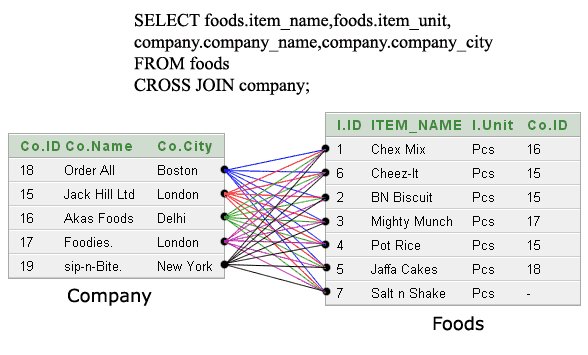
\includegraphics[width=0.8\textwidth]{cross.png}
	\caption{Cross Join Table Example}
	\label{fig:cross-png}
\end{figure}
Follow the coloured lines above to see how it cross joins. Each edge is a newly created tuple in the new table. To specify CROSS JOIN between two tables $R$ and $S$, we write
\begin{align*}
	R \text{ CROSS JOIN } S
\end{align*}
And similarly, for NATURAL JOIN
\begin{align*}
	R \text{ NATURAL JOIN }S
\end{align*}
Recall that queries create a table, therefore, we can also write
\begin{align*}
	query_1 \text{ CROSS JOIN } query_2 \\
	query_1 \text{ NATURAL JOIN } query_2
\end{align*}
\subsection{NATURAL JOIN}
$R$ NATURAL JOIN $S$ is equivalent to formatting the cross product of $R$ and $S$ and then looking for attributes of $ R$ that have the same name as attributes in $S$. Keep only tuples from product whose same-name-type attributes have same value. Only one of each set of duplicate columns is kept.
\begin{figure}[H]
	\centering
	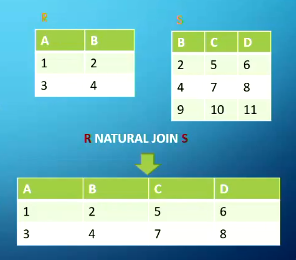
\includegraphics[width=0.45\textwidth]{njoin.png}
	\caption{NATURAL JOIN}
	\label{fig:njoin}
\end{figure}
\subsection{JOIN}
This is an extension to natural joins and it allows us to combine constraints (in WHERE) and a product in 1 operations. The syntax is
\begin{align*}
	R \text{ JOINS } S \text{ ON }<\text{condition}>
\end{align*}
$<\text{condition}>$ is used for selecting tuples. If operator is $=$ this is called an equi-join. For example,
\begin{align*}
	\text{Drinkers D JOIN Frequents F ON D.drinker = F.drinker}
\end{align*}
returns $(d,a,d,b)$ quadruples such that drinker $d$ lives at address $a$ and frequents teaRoom $b$.
The default join operator we have seen thus far is called inner join, for which there exist an explicit operator
\begin{align*}
	\text{SELECT } <\text{attList}> \text{ FROM } <\text{table1}> \text{ INNER JOIN } <\text{table2}> \text{ ON } <\text{expr}>;
\end{align*}
An inner join will combine the rows from $<\text{table1}>$ with the rows from $<\text{table2}>$ based on satisfying the ON boolean expression. The expression usually takes the form of a comparison between a column from table $1$ and a column from table $2$.
\subsection{INNER JOIN}
The inner join has the same functionality as
\begin{align*}
	\text{SELECT }*\text{ FROM student S, studentCourses C WHERE S.studentID = C.studentID}
\end{align*}
Explicitly using "Join" makes formatting more readable. Using 'ON' separates clauses that deal with sources of data i.e., belonging to FROM away from CLAUSES that deal with selection criteria
\subsection{OUTER JOIN}
Inner joins can "lose" information, become a tuple that doesn't join with any other relation disappears. Instead, outer join keeps this information and fills tuples that do not match with nulls if it is not matched when joining. You can further specify if you want to keep information on the left side or the right side, more specifically if you wanna keep information on the left table, then you type LEFT OUTER JOIN. You can further use the syntax $NATURAL$ to make the join natural, or use $ON$ syntax after the OUTER JOIN to specify when to join.
\end{document}
